\documentclass{article}

\usepackage[utf8]{inputenc}
\usepackage{graphicx}
\usepackage{listings}
\usepackage[a4paper, left=2cm, right=2cm, top=3cm, bottom=3cm]{geometry}
\usepackage{amsmath}
\title{Advaned Programming for HPC - Report 5}
\author{Dinh Anh Duc}

\begin{document}

\maketitle

\section*{Implementation}
\footnotesize\begin{lstlisting}

__global__ void gaussianNoShared(uchar3 *input, uchar3 *output, int imgWidth, int imgHeight){
        float gaussianBlur[7][7]={
            {0,   0,   1,   2,   1,   0,   0},
            {0,   3,   13,  22,  13,  3,   0},
            {1,   13,  59,  97,  59,  13,  1},
            {2,   22,  97,  159, 97,  22,  2},
            {1,   13,  59,  97,  59,  13,  1},
            {0,   3,   13,  22,  13,  3,   0},
            {0,   0,   1,   2,   1,   0,   0}
        };
        int col = threadIdx.x + blockIdx.x + blockDim.x;
        int row = threadIdx.y + blockIdx.y + blockDim.y;
        int tid = row * imgWidth + col;
        int sumR = 0;
        int sumG = 0;
        int sumB = 0;
        for (int j = 0; j < 7; j++) {
            for (int i = 0; i < 7; i++) {
                int cell_id = tid + i + j * imgWidth;
                sumR += input[cell_id].x * gaussianBlur[j][i];
                sumG += input[cell_id].y * gaussianBlur[j][i];
                sumB += input[cell_id].z * gaussianBlur[j][i];
            }
        }
    
        output[tid].x = sumR/1003;
        output[tid].y = sumG/1003;
        output[tid].z = sumB/1003;
}
__global__ void gaussianShared(uchar3 *input, uchar3 *output, int imgWidth, int imgHeight){
        float gaussianBlur[7][7]={
            {0,   0,   1,   2,   1,   0,   0},
            {0,   3,   13,  22,  13,  3,   0},
            {1,   13,  59,  97,  59,  13,  1},
            {2,   22,  97,  159, 97,  22,  2},
            {1,   13,  59,  97,  59,  13,  1},
            {0,   3,   13,  22,  13,  3,   0},
            {0,   0,   1,   2,   1,   0,   0}
        };
        
        int col = threadIdx.x + blockIdx.x + blockDim.x;
        int row = threadIdx.y + blockIdx.y + blockDim.y;
        int tid = row * imgWidth + col;

        __shared__ float gb[7][7];
        gb[threadIdx.x][threadIdx.y] = gaussianBlur[row][col];
        __syncthreads();

        int sumR = 0;
        int sumG = 0;
        int sumB = 0;
        for (int j = 0; j < 7; j++) {
            for (int i = 0; i < 7; i++) {
                int cell_id = tid + i + j * imgWidth;
                sumR += input[cell_id].x * gb[threadIdx.x][threadIdx.y];
                sumG += input[cell_id].y * gb[threadIdx.x][threadIdx.y];
                sumB += input[cell_id].z * gb[threadIdx.x][threadIdx.y];
            }
        }
    
        output[tid].x = sumR/1003;
        output[tid].y = sumG/1003;
        output[tid].z = sumB/1003;

}
void Labwork::labwork5_GPU(bool shared) {
    // Calculate number of pixels
    int pixelCount = inputImage->width * inputImage->height;	

    // Allocate CUDA memory    
    uchar3 *devInput;
    uchar3 *devOutput;
    cudaMalloc(&devInput, pixelCount);
    cudaMalloc(&devOutput, pixelCount);
    
    // Copy CUDA Memory from CPU to GPU
    cudaMemcpy(devInput, inputImage, pixelCount, cudaMemcpyHostToDevice);

    // Processing
    dim3 blockSize = dim3(32, 32);
    dim3 gridSize = ((int) ((inputImage->width + blockSize.x - 1)/blockSize.x), (int)((inputImage->height + blockSize.y - 1)/blockSize.y));
    if(shared == false){
        gaussianNoShared<<<gridSize, blockSize>>>(devInput, devOutput, inputImage->width, inputImage->height);
    }else{
        gaussianShared<<<gridSize, blockSize>>>(devInput, devOutput, inputImage->width, inputImage->height);
    }
    // Copy CUDA Memory from GPU to CPU
    cudaMemcpy(inputImage, devOutput, pixelCount, cudaMemcpyHostToDevice);

    // Cleaning
    //free(hostInput);
    cudaFree(devInput);
    cudaFree(devOutput);
}

\end{lstlisting}
\newpage
\section*{Result}
\begin{figure}[h]
\center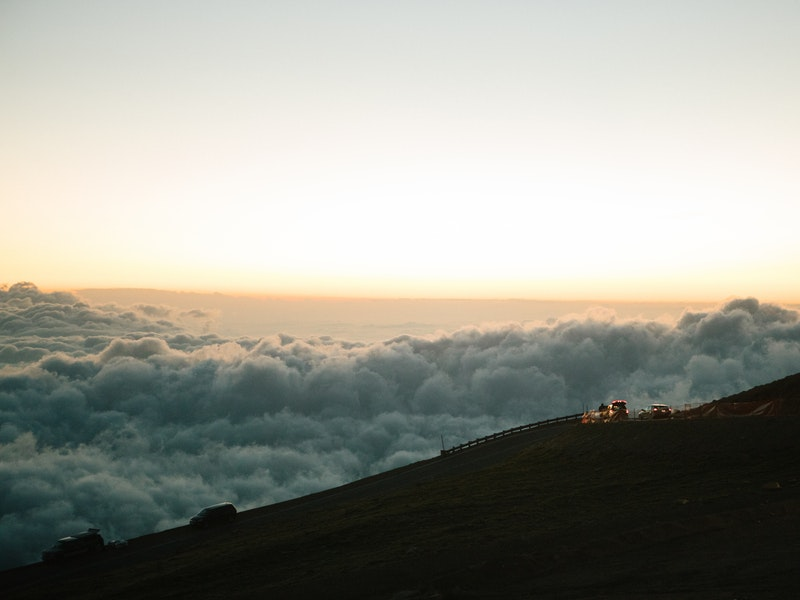
\includegraphics[scale=0.3]{./labwork/data/cloud.jpeg}
\caption{Original input image}
\end{figure}
\begin{figure}[h]
\center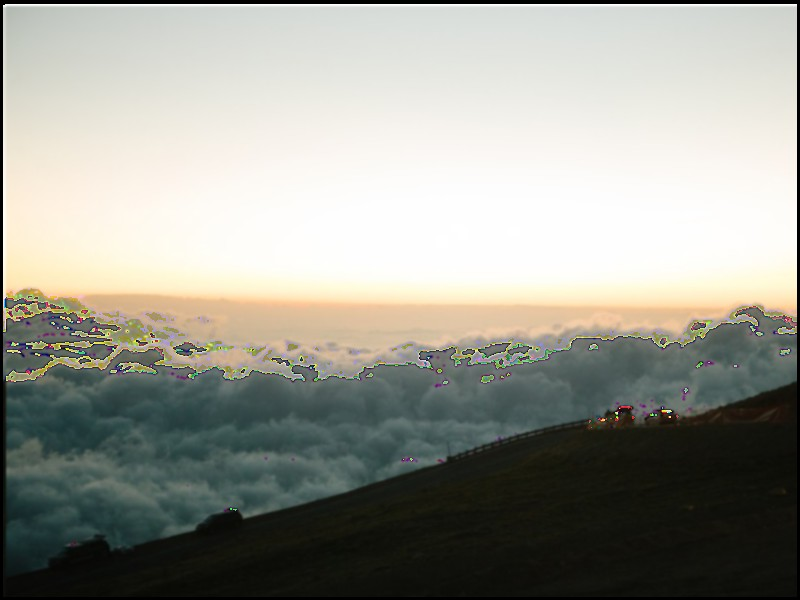
\includegraphics[scale=0.3]{./labwork/build/labwork5-gpu-out-shared.jpg}
\caption{Output image}
\end{figure}
\\
\section*{Without using shared memory mode}
\\
USTH ICT Master 2018, Advanced Programming for HPC.
\\
Warming up...
\\
Starting labwork 5
\\
labwork 5 ellapsed 222,5ms
\\
\section*{Using shared memory mode}
\\
USTH ICT Master 2018, Advanced Programming for HPC.
\\
Warming up...
\\
Starting labwork 5
\\
labwork 5 ellapsed 228.6ms

\end{document}

